\documentclass[12pt]{article}
\usepackage[margin=1in]{geometry}
\usepackage{amssymb}
\usepackage{amsmath}
\usepackage{amsthm}
\usepackage{amsfonts}
\usepackage[shortlabels]{enumitem}
\usepackage{mathtools} 
\usepackage{amscd}        % For simple commutative diagrams
\usepackage{graphicx}
\usepackage{rotating}     % To rotate figures, tables, ...
\usepackage{color}
\usepackage{pdfpages}
\usepackage{blkarray, bigstrut, multirow}
\usepackage{hyperref}


\begin{document}
\begin{titlepage}
    \begin{center}
        \vspace*{1cm}

        \textbf{Winning with Arclight Phoenix}

        \vspace{0.5cm}
        The way of the Bird

        \vspace{1.5cm}

        \textbf{Josh Mulloy}

        \vspace{0.8cm}

        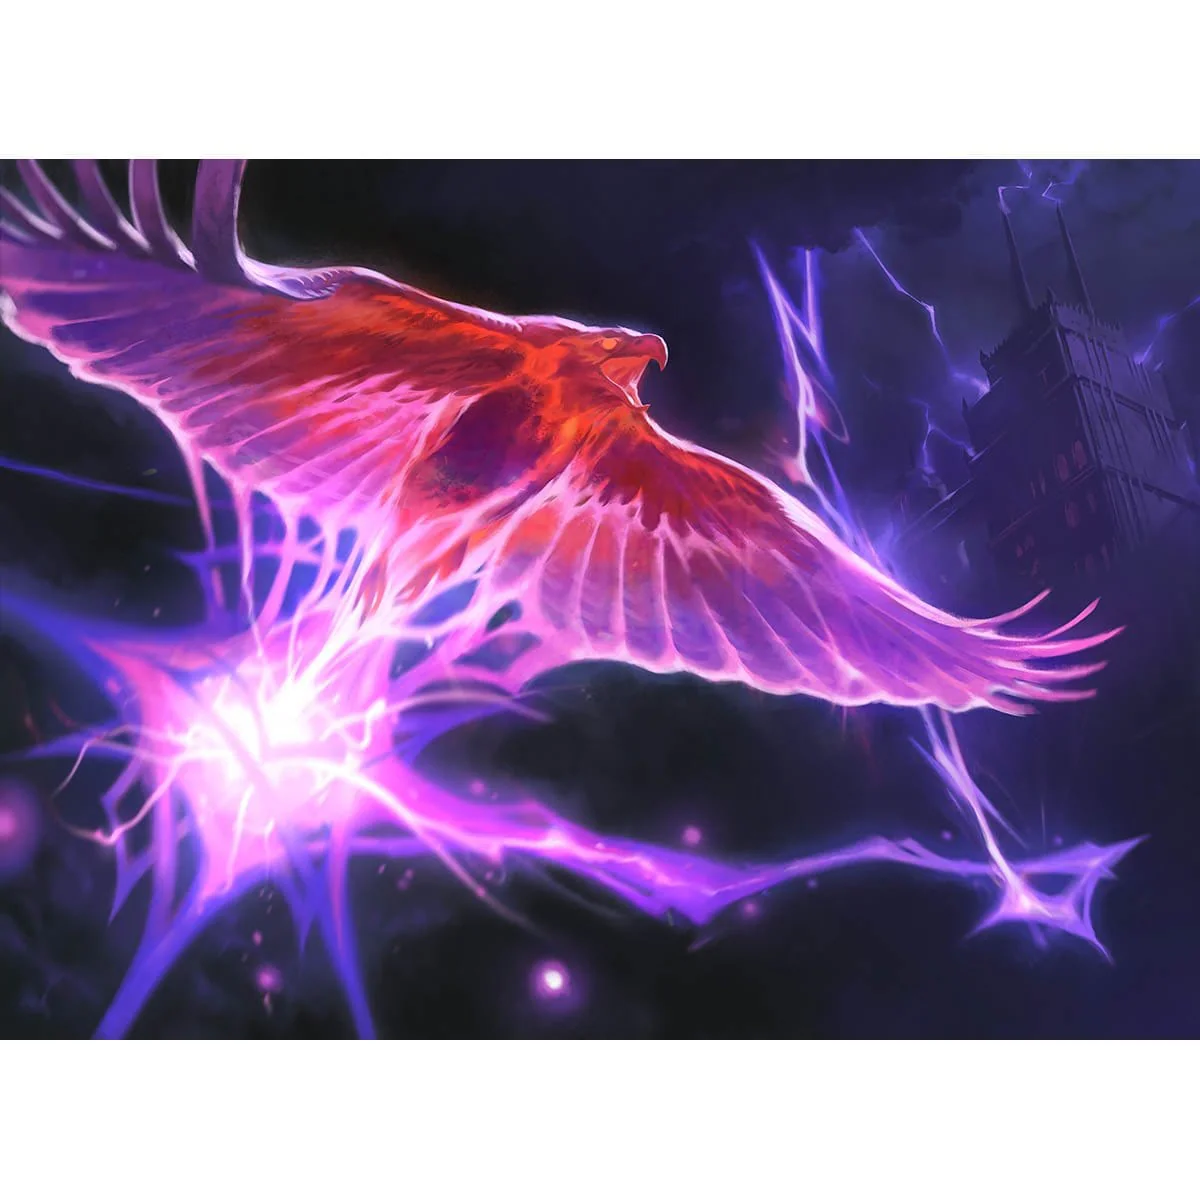
\includegraphics[width=0.7\textwidth]{arclight}

        \vfill

        A guide to playing arclight phoenix\\
        from a mid player
    \end{center}
\end{titlepage}

\tableofcontents

\clearpage
\section{Current List}
\begin{center}
    \href{https://www.mtggoldfish.com/deck/6561022#online}{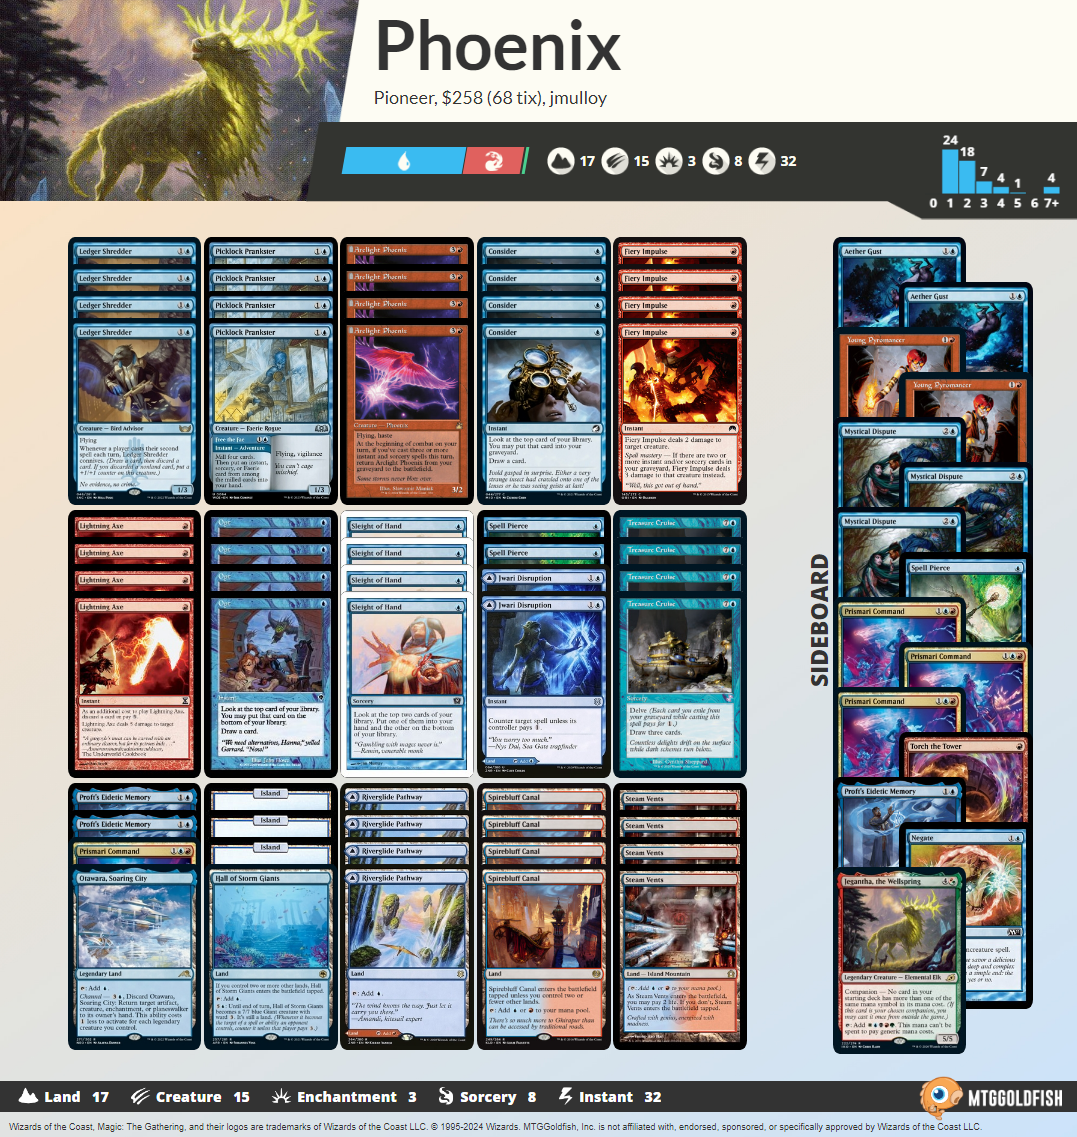
\includegraphics[width=1\textwidth]{decklist}}

    \href{https://www.mtggoldfish.com/deck/6561022}{https://www.mtggoldfish.com/deck/6561022}

    \vspace{0.5cm}

    \href{https://docs.google.com/spreadsheets/d/1DheUoGrQmpuwzbMDpPVJHcCrfe7UOyXSMSSkL8aXnv0/edit?usp=sharing}{Phoenix Matches (started tracking Aug 2024 [Challenge+ level]):}

    \href{https://docs.google.com/spreadsheets/d/1DheUoGrQmpuwzbMDpPVJHcCrfe7UOyXSMSSkL8aXnv0/edit?usp=sharing}{Spreadsheet Link}
\end{center}

\clearpage
\section{Why Phoenix?}
\subsection{Card Velocity}
Because phoenix plays 12 cantrips, 4 prankster, and 4 cruise, it is very easy to see most of your cards every game. This allows you to tune phoenix against basically any metagame, barring some pretty absurd things going on when phoenix is the clear best deck (like people registering waste not or lotus). Even when we are in one of these metas phoenix can still usually be tuned into a spot where we are fine into even these hate decks.

For example, with the newer prankster variants of phoenix we are able to play more spell pierce, depedning on the metagame. Some people even play a borrower in the main as a catch all that you can usually find when you need it. While I don't believe this to be better than just having Jegantha as a companion it speaks to how strong the ability to see so much of your deck is. This velocity is what makes the maindeck one ofs so interesting to me, something like maindeck primsari.

\subsection{Treasure Cruise}
I think a lot of people view phoenix as a deck that is just trying to put arclight phoenix into play as quickly as possible. While this is an admirable goal, it is not the main way that I play the deck. Often I would rather resolve a treasure crusie than put a single phoenix in play, and don't feel a strong urge to waste lightning axes because it will allow me to put phoenix into play.

As mentioned in the recent ban announcement, if phoenix manages to get another card banned in the format, its going to be cruise. The fact that we can chain cruise to go from empty handed to a full grip in a single turn for only two mana means that often even if an opponent manages to get a little ahead they will need to kill us fast.

\subsection{Low vs. High Resource Games}
Phoenix as a deck is really good at playing games where it always has things to be doing with its mana. I call these games \emph{high resource games}. They are the games where we cantrip a lot, resolve a few cruises, and maybe have a shredder that goes unanswered for a few turns. It is really hard for us to lose these kinds of games. The deck is just so capable of finding all the answers we need while also putting a ton of pressure on in these games that most decks have to somehow prevent us from getting into one of these games. The low resource games are the ones where we are paying four mana for phoenix and 6 mana for lightning axe. They are the games where we don't find many cantrips and can't seem to find or maybe even cast a crusie.

Most of the games we lose are going to be games where we aren't able to get one of these high resource games going. This is what makes a lot of the hate so good into phoenix, but also what makes some of the hate less good than people think. Things like hearse, rip, and to a lesser extent leyline of the void are the main ways that decks try to keep us from creating high resource games. Leyline is specifically called out here because often we are able to turn a leyline game into a high resource game, or, if they don't have it in their opener, we can do enough to have a critical mass before they play it. The hate that is less good at stopping us in these spots are things like go blank, cling to dust, damping sphere, and grafdiggers cage. Just one of these cards isn't going to be enough to stop us, and in the case of cling, sphere, and cage I think these cards are just straight up bad into phoenix.

\subsection{It is Fun}
Phoenix is an interesting deck because you are able to see so many of your cards every game. You are going to have a ton of opporunities to make decisions, even if most of them don't matter, and that definitely makes it feel like you have more agency in the games than you do. For some reason I think this makes the game more fun for me. Furthermore, you just get to take a ton of game actions, and what are we playing magic for if not to take as many game actions as possible.

\vspace{0.4em}
\noindent I also just really like casting treasure cruise, attacking with 3/2s, and taking game actions.

\clearpage
\section{The Details}
\subsection{Cantrip Sequencing}

\subsection{Playing Ledger Shredder}

\subsection{Graveyard Hate}

\subsection{Mulliganing}

\clearpage
\section{Card Choices}
\subsection{Main Deck Cards}
\label{sec:mainchoices}
\textbf{Jegantha:}
Much better than I expected it to be. Really good as just a card that can be put in hand to pitch to axe/shredder. Also fine as a beater in the low resource games.

\vspace{0.4em}
\noindent \textbf{Proft's Eidetic Memory:}
Trespass plays pretty poorly with prankster, while this plays really well. Pretty sure this is just better in the mirror too. Definitely reduces our combo potential, making it a bit more important to chip in for damage when possible compared to the old phoenix lists, but you can still use this to kill people out of nowhere.

\vspace{0.4em}
\noindent \textbf{Cantrips:}
Seen lists playing 3 sleight, 4 opt, 4 consider. Do not do this if you want to win.

\vspace{0.4em}
\noindent \textbf{Fiery Impulse:}
Depending on the meta you can trim one of the fiery impulses for a pierce or even a proft or prismari. I don't think the meta is currently in one of those places but if phoenix becomes extremely popular we could be living in that world.

\vspace{0.4em}
\noindent \textbf{Spell Pierce:}
A nice catch all against basically every deck. It often comes out even if it has targets but I like it for game ones. Also nice as a one mana piece of interaction.

\vspace{0.4em}
\noindent \textbf{Prismari Command:}
Does everything we want in the low resource games, while also dealing with most of the actually good hate against us. All 4 modes come up often. An important part of casting crusie in low resource games, acting as a quadruple lotus petal a lot of the time. Basically, it is a good anti hate card that also just plays really well in the games before, after, and during the hate. I like the idea of having one in the main, but this maybe should just be a sideboard card.

\vspace{0.4em}
\noindent \textbf{Lands:}
The way I see it, phoenix lists have 4 flex slots for lands, usually choosing between 3rd island, hall of storm giants, jwari disruption, mountain, and stormcarved coast. I like jwari as something to bridge the gap to a turn 3 shredder that also gives us the ability to sometimes steal games by sniping something or making our opponent sequence weird. Hall is similar, where it is just there to shore up some games that we could be losing without it, specifically the low resource ones. I haven't felt a lot of pressure on red sources in my lists so I don't play an additional red source in mountain or stormcarved, but not playing them means you have to be a bit more careful deciding whether to put your pathways on red.

\vspace{0.4em}
\noindent \textbf{Trespass/Iteration:}
See Proft section above. I just don't think we really need this anymore, especially because it prevents us from playing Jegantha. It's possible we want it as people start trying to beat us as it's the best way to steal game one sometimes. It usually ends up coming out even in these spots though, making me think I'd rather just be all in on proft.

\vspace{0.4em}
\noindent \textbf{Artist's Talent:}
I haven't played with this yet, it might be good but I doubt it. I like the cards I play impacting the board, and we don't really need help discarding cards. I don't really see a world where this is better than shredder.

\vspace{0.4em}
\noindent \textbf{Torch the Tower:}
This card isn't better than impulse in basically any mu, including the mirror. I can't see myself ever playing one main.

\subsection{Sideboard Cards}
\label{sec:sbchoices}
\noindent \textbf{Prismari Command:}
See above.

\vspace{0.4em}
\noindent \textbf{Mystical Dispute:}
Best counterspell we can play.

\vspace{0.4em}
\noindent \textbf{Negate:}
I think we need some hard permission. It's possible that we can play more now that we are using picklock instead of pieces, although the matchups where we want this we plan to play as a tempo deck.

\vspace{0.4em}
\noindent \textbf{Spell Pierce:}
Better than second negate as it can answer a rest in peace on the draw. Depending on their list we might even want this against some RB mid opponents.

\vspace{0.4em}
\noindent \textbf{Aether Gust:}
The best card we can have against Mono Green. Also has big implications against Niv and dromoka out of lotus. Notably it is fine against red and can help us answer Kroxa out of RB. Basically just a really good catch all.

\vspace{0.4em}
\noindent \textbf{Proft's Eidetic Memory:}
This is our best card in the mirror, as well as against most of the creature decks. It also helps agaist people packing excessive graveyard hate.

\vspace{0.4em}
\noindent \textbf{Young Pyromancer:}
Helps us when we want to switch to a tempo deck against decks like lotus and UW control. Also has big impact against the creature decks without reach, like humans and GW company (not angels). I think people often overboard it against decks like RB that makes it look worse than it is.

\vspace{0.4em}
\noindent \textbf{Torch the Tower:}
I currently have one of these as a ninth one mana removal spell against aggro decks. I still don't like the card but I think it may be a necessary evil.

\vspace{0.4em}
\noindent \textbf{Crackling Drake:}
I have always found crackling drake to be very awkward but necessary. Now that we have profts as our big card against graveyard hate, as well as prismari to better answer hate, I think it is less needed. It is just super awkward that you tap out to play it and your opponent can often kill it and advance their board putting you way behind, although this is offset by them usually dying if you untap. I think we just no longer need it, especially because proft lets us have Jegantha post board in the matchups where it's best.

\vspace{0.4em}
\noindent \textbf{Thing in the Ice:}
A very good card against green and company decks (to the extent it can be good into skyclave). I don't think it's that good into basically anything else, with it being quite a bit worse than just another removal spell against mono red and mono white. The fact that the green decks can't slow down our graveyard plan as much anymore makes me want to play this much less, although it is quite good against angels if that makes a comeback.

\vspace{0.4em}
\noindent \textbf{Brotherhood's End:}
In the past we have used this card as an answer to artifact hate and trespasser out of RB mid. It's also fine as a wrath against the aggro decks, although it has diminishing returns against mono white and mono red. If the GW company decks become more popular it likely gets better but I'm unconvinced it will be better than something like Thing in the Ice that lets us keep Jegantha.

\vspace{0.4em}
\noindent \textbf{Anger of the Gods:}
Without Amalia in the format anymore this card is significantly worse than brotherhood's end.

\vspace{0.4em}
\noindent \textbf{Ashiok, Dream Render:}
Probably the best hate card we can play. It is quite good in the mirror, although weak to dispute and pierce, while also having good interactions against Lotus and Niv. Against the mirror I think it is better to be on the proft side than the Ashiok side, and against Lotus and Niv I would rather just be trying to tempo them out. The fact this turns off Jegantha is a bit less relevant as the matchups Ashiok is good aren't really the matchups where Jegantha is best. For now I think I'm going to leave Ashiok out but I could see wanting it.


\clearpage
\section{Matchups and Sideboarding}
\subsection{Phoenix Mirror}

\subsection{RB Mid}

\subsection{Mono Green}

\subsection{Lotus Combo}

\subsection{Spirits}

\subsection{UW/UB Control}

\subsection{Niv/Enigmatic}

\subsection{Ensoul}

\subsection{Red Aggro}

\subsection{GB Food}

\subsection{RB Sac}

\subsection{GW Company}

\subsection{Angels}

\end{document}